\documentclass[12pt]{article}   	% use "amsart" instead of "article" for AMSLaTeX format
\usepackage{amssymb}
\usepackage{amsmath}
\usepackage{graphicx}%
\usepackage{amsfonts}%
%\usepackage{float}
\usepackage{natbib}
\usepackage{floatrow}
\bibliographystyle{agsm}
\setcitestyle{authoryear,open={(},close={)},aysep={}}
\usepackage{xr}
\usepackage{hyperref}
\usepackage{subcaption}
\captionsetup[subfigure]{labelformat=empty}
\usepackage{sidecap}

\usepackage{multirow}
\renewcommand{\baselinestretch}{1.0}
\setlength{\oddsidemargin}{0in} \setlength{\textwidth}{6.5in}
%SetFonts
\newcommand{\blam}{ \mbox{\boldmath $ \lambda $} }
\newcommand{\bet}{ \mbox{\boldmath $ \eta $} }
\newcommand{\btau}{ \mbox{\boldmath $ \tau $} }
\newcommand{\bome}{ \mbox{\boldmath $ \omega $} }
\newcommand{\bbet}{ \mbox{\boldmath $ \beta $} }
\newcommand{\bbeta}{ \mbox{\boldmath $ \beta $} }
\newcommand{\balph}{ \mbox{\boldmath $ \alpha $} }
\newcommand{\balpha}{ \mbox{\boldmath $ \alpha $} }
\newcommand{\bphi}{ \mbox{\boldmath $\phi$}}
\newcommand{\bzeta}{ \mbox{\boldmath $\zeta$}}
\newcommand{\bkap}{ \mbox{\boldmath $\kappa$}}
\newcommand{\bkappa}{ \mbox{\boldmath $\kappa$}}
\newcommand{\beps}{ \mbox{\boldmath $\epsilon$}}
\newcommand{\bepsilon}{ \mbox{\boldmath $\epsilon$}}
\newcommand{\bthet}{ \mbox{\boldmath $ \theta $} }
\newcommand{\btheta}{ \mbox{\boldmath $ \theta $} }
\newcommand{\bnu}{ \mbox{\boldmath $\nu$} }
\newcommand{\bmu}{ \mbox{\boldmath $\mu$} }
\newcommand{\bOmega}{ \mbox{\boldmath $\Omega$} }
\newcommand{\bGam}{ \mbox{\boldmath $\Gamma$} }
\newcommand{\bSig}{ \mbox{\boldmath $\Sigma$} }
\newcommand{\bSigma}{ \mbox{\boldmath $\Sigma$} }
\newcommand{\bPhi}{ \mbox{\boldmath $\Phi$} }
\newcommand{\bThet}{ \mbox{\boldmath $\Theta$} }
\newcommand{\bTheta}{ \mbox{\boldmath $\Theta$} }
\newcommand{\bDel}{ \mbox{\boldmath $\Delta$} }
\newcommand{\bDelta}{ \mbox{\boldmath $\Delta$} }
\newcommand{\bnabla}{ \mbox{\boldmath $\nabla$} }
\newcommand{\bLam}{ \mbox{\boldmath $\Lambda$} }
\newcommand{\bLambda}{ \mbox{\boldmath $\Lambda$} }
\newcommand{\bLambdasub}{ \scriptsize{\bLambda}}
\newcommand{\bgam}{ \mbox{\boldmath $\gamma$} }
\newcommand{\bgamma}{ \mbox{\boldmath $\gamma$} }
\newcommand{\brho}{ \mbox{\boldmath $\rho$} }
\newcommand{\bdel}{ \mbox{\boldmath $\delta$} }
\newcommand{\bdelta}{ \mbox{\boldmath $\delta$} }
\newcommand{\bvarphi}{ \mbox{\boldmath $\varphi$} }
\newcommand{\bsigma}{ \mbox{\boldmath $\sigma$} }
\newcommand{\boeta}{ \mbox{\boldmath $\eta$} }
\newcommand{\bpi}{ \mbox{\boldmath $\pi$} }
\newcommand{\bpsi}{ \mbox{\boldmath $\psi$} }
\newcommand{\bzero}{\textbf{0}}
\newcommand{\bone}{\textbf{1}}
\newcommand{\bZ}{\textbf{Z}}
\newcommand{\bz}{\textbf{z}}
\newcommand{\ba}{\textbf{a}}
\newcommand{\bA}{\textbf{A}}
\newcommand{\bb}{\textbf{b}}
\newcommand{\bB}{\textbf{B}}
\newcommand{\bc}{\textbf{c}}
\newcommand{\bC}{\textbf{C}}
\newcommand{\bd}{\textbf{d}}
\newcommand{\bD}{\textbf{D}}
\newcommand{\be}{\textbf{e}}
\newcommand{\bE}{\textbf{E}}
\newcommand{\bbf}{\textbf{f}}
\newcommand{\bF}{\textbf{F}}
\newcommand{\bk}{\textbf{k}}
\newcommand{\bK}{\textbf{K}}
\newcommand{\bh}{\textbf{h}}
\newcommand{\bH}{\textbf{H}}
\newcommand{\bi}{\textbf{i}}
\newcommand{\bI}{\textbf{I}}
\newcommand{\bg}{\textbf{g}}
\newcommand{\bG}{\textbf{G}}
\newcommand{\bJ}{\textbf{J}}
\newcommand{\bL}{\textbf{L}}
\newcommand{\bm}{\textbf{m}}
\newcommand{\bM}{\textbf{M}}
\newcommand{\bn}{\textbf{N}}
\newcommand{\bN}{\textbf{N}}
\newcommand{\bO}{\textbf{O}}
\newcommand{\bp}{\textbf{p}}
\newcommand{\bP}{\textbf{P}}
\newcommand{\bq}{\textbf{q}}
\newcommand{\bQ}{\textbf{Q}}
\newcommand{\bs}{\textbf{s}}
\newcommand{\bS}{\textbf{S}}
\newcommand{\bt}{\textbf{t}}
\newcommand{\bT}{\textbf{T}}
\newcommand{\bu}{\textbf{u}}
\newcommand{\bU}{\textbf{U}}
\newcommand{\bv}{\textbf{v}}
\newcommand{\bV}{\textbf{V}}
\newcommand{\bw}{\textbf{w}}
\newcommand{\bW}{\textbf{W}}
\newcommand{\bx}{\textbf{x}}
\newcommand{\bX}{\textbf{X}}
\newcommand{\by}{\textbf{y}}
\newcommand{\bY}{\textbf{Y}}
\newcommand{\br}{\textbf{r}}
\newcommand{\bR}{\textbf{R}}
\newcommand{\iidsim}{\overset{\text{iid}}{\sim} }
\newcommand{\indsim}{\stackrel{\mbox{\tiny indep}}{\sim}}
\newcommand{\set}{\overset{\text{set}}{=} }

\newcommand{\E}{\mathbb{E}}

\usepackage{xcolor}
\xdefinecolor{custom_red}{rgb}{0.58, 0.32, 0.32} % Marsala
%% SOLUTIONS -- must comment one out
% OFF
%\newcommand{\soln}[2]{\vspace{0cm}}{}
% ON 
\newcommand{\soln}[2]{\textit{\textcolor{custom_red}{#2}}}{}

\usepackage[headheight=65pt,tmargin=65pt,headsep=5pt, margin = 1in]{geometry}

\usepackage{fancyhdr}
\pagestyle{fancy}

\lhead{STAT 201}
\rhead{Solutions}
\chead{\Large{Practice Problems}}
\renewcommand{\headrulewidth}{0.4pt}
\renewcommand{\footrulewidth}{0pt}
\begin{document}

\subsection*{Intro Hypothesis Testing }

\begin{enumerate}
\item
  For each of the research statements below, determine whether it
  represents a null hypothesis claim or an alternative hypothesis claim.

  \begin{enumerate}
  \item
    The number of hours that grade-school children spend doing homework
    predicts their future success on standardized tests. \soln{}{Alternative}
  \item
    King cheetahs on average run the same speed as standard spotted
    cheetahs. \soln{}{Null}
  \item
    For a particular student, the probability of correctly answer a
    5-option multiple choice test is larger than 0.2 (i.e.~better than
    guessing)  \soln{}{Alternative}
  \item
    The probability of getting in a car accident is the same if using a
    cell phone then if not using a cell phone. \soln{}{Null}
  \end{enumerate}
   
  \item
  Write out the null and alternative hypotheses in words and also in
  statistical notation for each of the following situations. When
  writing in statistical notation, be sure to define quantities in
  context.

  \begin{enumerate}
  \item
    New York is known as ``the city that never sleeps''. A random sample
    of 25 New Yorkers were asked how much they sleep they get per night.
    Does these data providing convincing evidence that New Yorkers on
    average sleep less than 8 hours per night?
    
    \soln{}{$H_{0}: \mu = 8$ (On average New Yorkers sleep 8 hours a night) versus $H_{A}: \mu < 8$ (On average New Yorkers sleep less than 8 hours a night), where $\mu$ is the mean hours of sleep New Yorkers receive. }
    
  \item
    A study suggests that 25\% of 25 year-olds have gotten married. You
    believe that this is incorrect and decide to collect your own data
    to conduct a hypothesis test.
    
        \soln{}{$H_{0}: p = 0.25$ (True proportion of 25 year-olds who have gotten married is 25\%) versus $H_{A}: p \neq 0.25$ (True proportion of 25 year-olds who have gotten married is not 25\%) }
        
  \end{enumerate}
\item
  A Survey USA poll conducted in Seattle, WA in May 2021 reports that of
  the 650 respondents (adults living in this area), 159 support
  proposals to defund police departments.

  \begin{enumerate}
  \item
    A journals writing a news story on the poll results wants to use the
    headline: ``More than 1 in 5 adults living in Seattle support
    proposals to defund police departments''. You caution the journalist
    that they should first conduct a hypothesis test to see if the poll
    data provide convincing evidence for this claim. Write the
    hypotheses for this test using proper notation, defining any
    necessary quantities.
    
    \soln{}{$H_{0}: p = 0.20$ versus $H_{A}: p > 0.20$ where $p$ is the true proportion of Seattle adults who support proposals to defund.}
  \item
    Describe in words a simulation scheme that would be appropriate for
    this situation. Also describe how the p-value can be calculated
    using the simulation results.
    
    \soln{}{Example solution: . Take 100 cards, 20
black cards representing those who support proposals to defund police departments
and 80 red cards representing those who do not. Shuffle the cards and draw with
replacement (shuffling each time in between draws to get our ``infinite population") 650 cards representing the 650
respondents to the poll. After each iteration, calculation $\hat{p}_{sim}$, the  proportion of black cards which represents the simulated proportion of adults in favor. The p-value will be the proportion of simulations where $\hat{p}_{sim} \geq 0.245$.}
    
  \item
    The histogram below shows the distribution of 1000 simulated
    proportions under \(H_{0}\). Estimate the p-value using the plot and
    use it to evaluate your hypotheses (i.e.~make a conclusion). Assume
    a significance level of 0.05.

    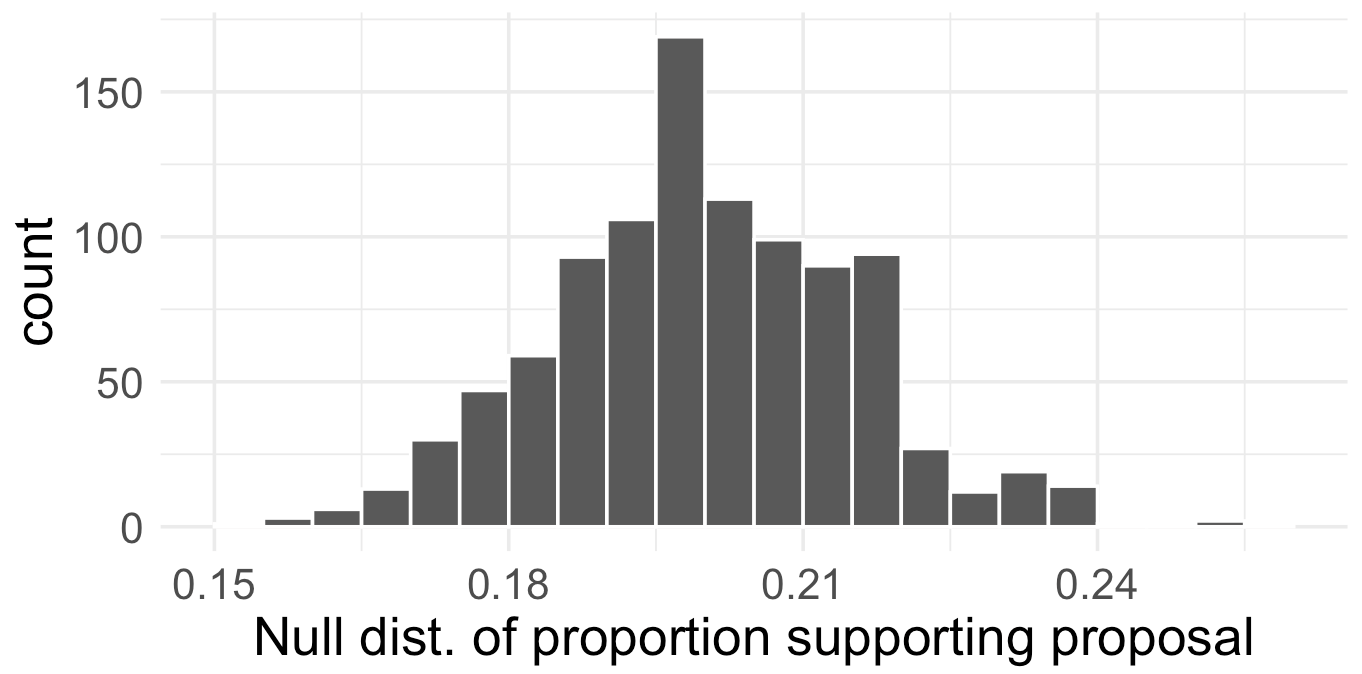
\includegraphics[scale = 0.4]{images/13-defund.png}
    
    \soln{}{There is only one simulated proportion that is at least 0.245, therefore the approximate p-value is 0.001. Since $0.001 < 0.05$, reject $H_{0}$. The data provide convincing evidence that the proportion of Seattle adults who support proposals to
defund police departments is greater than 0.20.}
    
  \end{enumerate}
  
  \item
  A study conducted in 2020 found that the U.S. adjusted divorce rate
  was 14 per 1000 married women. Joe is suspicious and disagrees with
  the stated divorce rate. Joe somehow collected data from 323 married
  or previously-married women, and asked them if they had a divorce in
  2020. 55 of the women responded that they indeed had a divorce in
  2020.

  \begin{enumerate}
  \item
    Write out the hypotheses corresponding to this scenario.
    
    \soln{}{$H_{0}: p = 0.14$ versus $H_{A}: p \neq 0.14$ where $p$ is the true divorce rate among married women.}
    
      \item
    Describe in words a simulation scheme that would be appropriate for
    this situation. Also describe how the p-value can be calculated
    using the simulation results.
    
    \soln{}{Similar to previous problem.}
    
  \item
    The histogram below shows the distribution of 100 simulated
    proportions under \(H_{0}\). Estimate the p-value using the plot and
    use it to evaluate Joe's hypotheses (i.e. make a conclusion). Assume
    a significance level of 0.05.

    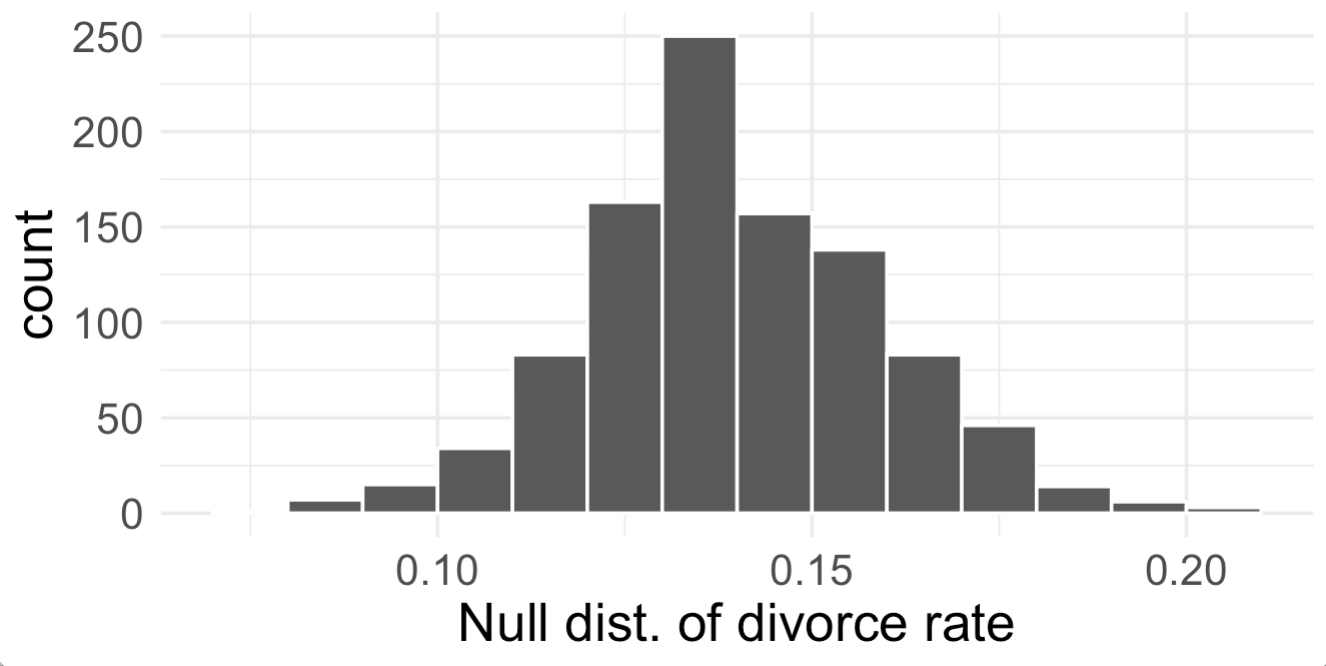
\includegraphics[scale = 0.4]{images/13-divorce.png}
    
    \soln{}{The observed proportion was $\hat{p}_{obs}  = 55/323 = 0.17$. Since the alternative is two-sided, the p-value is approximately 0.13.  Since this is larger than 0.05, fail to reject. The data do not provide convincing evidence that the divorce rate amount married women is different from 0.14.}
  \item
    Joe has some free time and also created a 90\% bootstrap confidence
    interval for the divorce rate.

    He obtained the following interval: (0.136, 0.207). Interpret this
    interval in context.
    
    \soln{}{Joe is 90\% confidence that the true divorce rate among married women is between 0.136 and 0.207.}
  \item
    Based on this interval, would it be appropriate for Joe to conclude
    that the study's reported rate was wrong? Explain your reasoning.
    
    \soln{}{No!  0.14 is included in the interval, so it is a plausible value.}
    
  \item
    How do your conclusions from (c) and (e) compare? 
    
    \soln{}{They agree!}
  \end{enumerate}
\end{enumerate}
  
 
 \subsection*{Randomization}
 
 \begin{enumerate}
\item
  The Stanford University Heart Transplant Study was conducted to
  determine whether an experimental heart transplant program increased
  lifespan. Each patient entering the program was designated an official
  heart transplant candidate, meaning that they were gravely ill and
  would most likely benefit from a new heart. Some patients got a
  transplant and some did not. The variable \texttt{transplant}
  indicates which group the patients were in: treatment (received
  transplant) or control (no transplant). The variable \texttt{survived}
  indicates whether the patient was alive at the end of the study or
  died. Of the 34 patients in the control group, 30 died. Of the 69
  people in the treatment group, 45 died.

  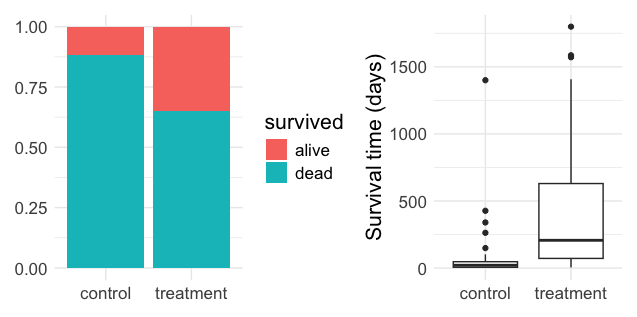
\includegraphics[scale = 0.4]{images/14-heart-transplant-eda.png}

  \begin{enumerate}
  \item
    What do the two plots above suggest about 1) if survival is
    independent of receiving a transplant and 2) the efficacy of heart
    transplants? Explain your reasoning.
    
    \soln{}{Proportion of patients who are alive at the end of the study is higher in the treatment
group than in the control group. These data suggest that survival is not independent
of whether the patient got a transplant.}
    
   
  \item
    What proportion of patients in the treatment group and the control
    group died?
    
    \soln{}{Proportion of patients who in the treatment group who are deceased: $45/69 = 0.652$.
Proportion of patients who in the control group who are deceased: $30/34 = 0.882$.}

  \item
    Write out a null and alternative hypothesis for investigating
    whether there is statistically significant evidence that the
    treatment is effective.
    
    \soln{}{$H_{0}:$  group (treatment or control) and survival outcomes are independent (i.e. the treatment does not affect death rate. $H_{A}$: the group and survival outcome are dependent, and specifically, the treatment is effective (decreases death rate).}
  \item
    The paragraph below describes the set up for a randomization test if
    we did not have access to software. Fill in the blanks with a number
    or phrase using your answers to (b) and (c) for guidance:

    We write the word \soln{}{``alive" (or something similar)} on  \soln{}{28} cards representing
    patients who were alive at the end of the study, and \soln{}{``dead" (or something similar)} on
    \soln{}{75} cards representing the patients who were not. Then we
    shuffle these cards and split them into two groups: one group of
    size \soln{}{69} representing treatment, and one group of size
    \soln{}{34} representing \soln{}{control}. We calculate the
    difference between the proportion of \soln{}{``died"} cards in the
    treatment and control groups (treatment - control) and record this
    value. We repeat this 1000 times to build a distribution centered at
   \soln{}{0}. This is called the  \soln{}{null} distribution.
    Lastly, we calculate the proportion of simulations where the
    simulated difference in proportions are  \soln{}{less than or equal to -0.23}. If this
    proportion is low, we conclude that that it is \soln{}{unlikely}
    to have observed our data by chance assuming \soln{}{$H_0$ is true}.
    
  \item
    What do the simulation results shown below suggest about the
    effectiveness of heart transplants?

    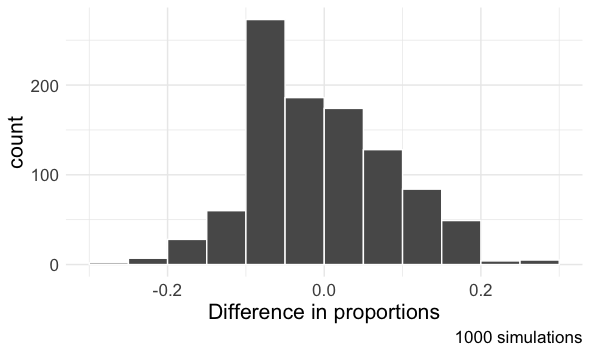
\includegraphics[scale=0.4]{images/14-heart-transplant-null.png}
    
    \soln{}{The $p$-value is approximately 0, which suggest that the transplant program is effective. }
  \item
    Suggest a more informative x-axis label for the plot above.
   
   \soln{}{Include (treatment - control)}
  \end{enumerate}
\item
  Understanding cultural differences in tobacco use across different
  demographic groups can lead to improved health care education and
  treatment. A recent study dis-aggregated tobacco use across Asian
  American ethnic groups, including Asian-Indian (n = 4373), Chinese (n
  = 4736), and Filipino (n = 4912), in comparison to non-Hispanic Whites
  (n = 275025). The number of current smokers in each group at the time
  of study was reported as:

  \begin{itemize}
  \item
    Asian-Indian: 223
  \item
    Chinese: 279
  \item
    Filipino: 609
  \item
    non-Hispanic Whites: 50880
  \end{itemize}

  To determine whether the proportion of Asian-Indian Americans who are
  current smokers is different from the proportion of Chinese Americans
  who are smokers, a randomization simulation was performed.

  \begin{enumerate}
  \item
    Using both symbols and words, provide the parameter and statistic of
    interest for this study. Do you know the numerical value of either
    the parameter or statistic of interest? If so, provide it.
    
    \soln{}{$p_{AI} - p_{C}$ where $p_{AI}$ is the proportion of Asian-Indian Americans who smoke, and $p_{C}$ is the proportion of Chinese Americans who smoke. The parameter is the true difference (Asian-Indian - Chinese) in proportions of these groups, and the statistic is the observed difference. We don't know the parameter, by the statistic is $\hat{p}_{AI} - \hat{p}_{C} = 223/4373 - 279/4736 = -0.008.$}
  \item
    The histogram below provides the simulated null distribution
    obtained from 1000 repetitions. Estimate the standard error.

    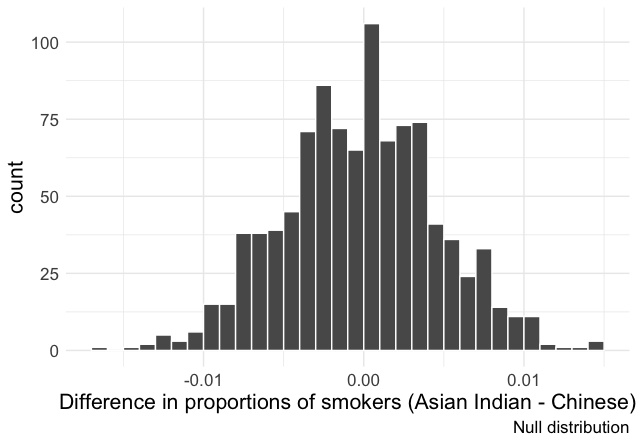
\includegraphics[scale = 0.4]{images/14-asian-tobacco-null.png}
  \item
    Consider the hypothesis test to determine if there is a difference
    in proportion of Asian-Indian Americans as compared to Chinese
    Americans who are current smokers. Write out the null and
    alternative hypotheses, and estimate a p-value using the
    randomization histogram from (b). If the significance level is
   \(\alpha = 0.05\), what is your decision and conclusion in the
    context of the problem?
    
    \soln{}{$H_{0}: p_{AI} - p_{C} = 0$ versus $H_{A}: p_{AI} - p_{C} \neq 0$. I would estimate about 100 simulations resulted in simulated difference in proportions less than or equal to the observed $-0.008$ or greater than equal to $0.008$. So i would fail to reject $H_0$. The data do not provide convince evidence that the true difference in
proportion of current smokers is different across the two ethnic groups. }
    
    
  \item
    Now consider the following bootstrap distribution of the difference
    in sample proportions of current smokers (Filipino Americans minus
    Chinese Americans) in 1000 repetitions. Find a 95\% bootstrap
    confidence interval for the true difference in the proportion of
    current smokers in the population. Interpret the interval in the
    context of the problem, assuming our sample is representative.

    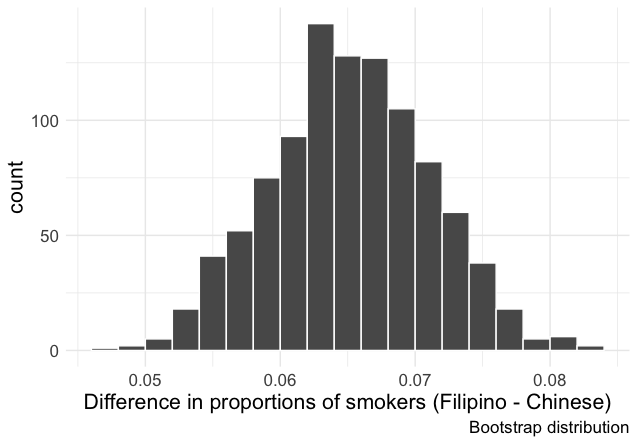
\includegraphics[scale = 0.4]{images/14-asian-tobacco-boot.png}
    
    \soln{}{A (symmetric) 95\% bootstrap confidence interval is approximately $(0.054, 0.076)$. Thus, we are 95\% confident that the proportion of Filipino Americans who smoke is between 0.054 and 0.076 higher than that of Chinese Americans.  }
  \end{enumerate}
\end{enumerate}

\subsection*{HT Basics}

\begin{enumerate}
\item
  For each of the statements (a) - (d), indicate if they are true or
  false interpretation of the following confidence interval. If false,
  provide or a reason or correction to the misinterpretation.

  ``You collect a large sample and calculate a 95\% confidence interval
  for the average number of cans of soda consumed annually per adult to
  be (440, 520), i.e.~on average, adults in the US consume just under
  two cans of soda per day''.

  \begin{enumerate}

  \item
    95\% of adults in the US consume between 440 and 520 cans of soda
    per year. \soln{}{False.The interval is for the parameter (a number which describes the population),
not for individual observational units. }
  \item
    There is a 95\% chance that the true population average per adult
    yearly soda consumption is between 440 and 520 cans. \soln{}{False. Although unknown, the parameter is either in the interval or it is not (so
either with probability zero or probability one).}
  \item
    The true population average per adult soda consumption is between
    440 and 520 cans, with 95\% confidence. \soln{}{True}
  \item
    The average soda consumption of the people who were is sampled is
    between 440 and 520 cans of soda per year, with 95\% confidence. \soln{}{The sample mean is always inside the interval (it is the center!). We are
100\% confident that the sample mean is in the interval}
  \end{enumerate}
\item
  A food safety inspector is called upon to investigate a restaurant
  with a few customer reports of poor sanitation practices. The food
  safety inspector uses a hypothesis testing framework to evaluate
  whether regulations are not being met. If the inspector determines the
  restaurant is in gross violation, its license to serve food will be
  revoked.

  \begin{enumerate}
  \item
    Write the hypotheses in words (no population parameters necessary).
    
    \soln{}{$H_0$: restaurant means food safety regulations. $H_{A}$: restaurant does not meet food safety regulations.}
  \item
    What is a Type I error in this context?
    
     \soln{}{The food safety inspector concludes that the restaurant does not meet food safety
and sanitation regulations and shuts down the restaurant when the restaurant is
actually safe.}
  \item
    What is a Type II error in this context?
    
    \soln{}{The food safety inspector concludes that the restaurant meets food safety and sanitation regulations and the restaurant stays open when the restaurant is actually
not safe.}
  \item
    Which error is more problematic for the restaurant owner? For the
    diners? Why?
    
    \soln{}{A Type I error may be more problematic for the restaurant owner since his restaurant gets shut down even though it meets the food safety and sanitation regulations. A Type II error may be more problematic for diners since the restaurant deemed
safe by the inspector is actually not.}
  \item
    Do you think the diners would prefer a higher or lower significance
    level \(\alpha\) compared to what the restaurant owner prefers? 
    Explain.
    
    \soln{}{A diner would probably prefer strong evidence as any indication of evidence might mean there
may be an issue with the restaurant meeting food safety regulations,
and diners would rather a restaurant that meet the regulations get shut down than a
restaurant that doesn’t meet the regulations not get shutdown}
  \end{enumerate}
\item
  Consider the following simple random sample
  \(x = (47, 4, 92, 47, 12, 8)\).

  Which of the following sets of values could be a possible bootstrap
  sample from the observe data above? If a set of values could not be a
  bootstrap sample, determine why not.

  \begin{enumerate}
  \item
    \((47, 47, 47, 47, 47, 47)\) \soln{}{Yes}
  \item
    \((92, 4, 13,8, 47, 4)\) \soln{}{No! 13 was not in original sample.}
  \item
    \((4, 8, 12, 12, 47)\) \soln{}{No; we need a resample of same size as original.}
  \item
    \((12, 4, 8, 8, 92, 12)\) \soln{}{Yes}
  \item
    \((8, 47, 12, 12, 8, 4, 92)\) \soln{}{No; we need a resample of same size as original.}
  \end{enumerate}
\item
  For each of the following statements (a)-(e), indicate if they are a
  true or false interpretation of the p-value. If false, provide a
  reason or correction to the misinterpretation.

  ``You are wondering if the average amount of cereal in a 10 oz. cereal
  box is greater than 10 oz. You collect 50 boxes of cereal marketed as
  10 oz, conduct simulation-based hypothesis test, and obtain a p-value
  of 0.23.''

  \begin{enumerate}
  \item
    The probability that the average weight of all cereal boxes is 10
    oz. is 0.23. 
    
    \soln{}{False. The p-value describes a probability about data, not a probability about a
parameter.}
  \item
    The probability that the average weight of all cereal boxes is
    something greater than 10 oz. is 0.23.
    
    \soln{}{False. The p-value describes a probability about data, not a probability about a
parameter.}
    
  \item
    Because the p-value is 0.23, the average weight of all cereal boxes
    is 10 oz.
    
    \soln{}{False. The p-value describes a probability about data, not a probability about a
parameter.}
 
  \item
    Because the p-value is small, the population average must be just
    barely about 10 oz.
    
    \soln{}{False; the p-value doesn't convey information about certainty and ``just barely".}
  \item
    If $H_{0}$ is true, the probability of observing another sample
    with an average as or more extreme as the data is 0.23.
    
    \soln{}{True.}
    
  \end{enumerate}
\end{enumerate}

\subsection*{Normal}

\begin{enumerate}
\item
  True or false? Briefly explain why.

  Among applicants to one law school, the average LSAT was about 169,
  the standard deviation about 9, and the highest score was 178. The
  distribution of the LSAT scores follows the normal curve.
  
  \soln{}{False: 68-96-99.7 rule.}
\item
  In a law school class, the entering students averaged 160 on the LSAT.
  The variance was 64. The histogram of LSAT scores followed the normal
  curve reasonable well.

  \begin{enumerate}
  \item
    About what percentage of the class scores below 152?
    
    \soln{}{Since variance is 64, standard deviation is 8. Score of 152 is one standard deviation below mean. Using 68-95-99.7 rule and symmetry, this is approximately $0.5 - 0.34 = 0.16$.}
  \item
    One student was 0.5 standard deviations above average on the LSAT.
    About what percentage of the students had lower scores than he did?
    
    \soln{}{pnorm(164, 160, 8) = pnorm(0.5) = 0.691}
  \end{enumerate}
\end{enumerate}

\begin{enumerate}
\item
  Weights of 10-year-old girls are known to be Normally distributed with
  mean of 70 pounds and standard deviation of 13 pounds. Find the
  probability that a 10-year-old girl  weighs between 60 and 85
  pounds two ways:

  \begin{enumerate}
  \item
    Optional, but helpful: draw a sketch of the curve and shade in the
    region of interest.
  \item
    Write the probability of interest in \(P()\) form. Then write the
    \texttt{R} code necessary to find this probability, and actually
    execute the code to obtain the probability.
    
    \soln{}{$P(60 \leq X \leq 85)$ where $X$ the weight of a 10 year old girl. Code: pnorm(85, 70, 13) - pnorm(60, 70, 13) = 0.655.}
    
  \item
    Confirm your solution in (b) by transforming to z-scores first, then
    using code again to obtain the probability.
    
    \soln{}{pnorm(15/13) - pnorm(-10/13 ) }
  \end{enumerate}
\item
  Consider the same scenario as in 3. Without using any code than what
  is provided below, find the 60th percentile for the weight of
  10-year-old girls.

\begin{verbatim}
qnorm(0.6, mean = 0, sd = 1) = 0.2533471
\end{verbatim}

	\soln{}{Working backwards: $0.253 = \frac{x - 70}{13}$, so $x = 73.419$ pounds.}

\item
  The length of human pregnancies from contraception to birth varies
  according to a distribution that is approximately normal with mean 266
  days and standard deviation 16 days. Without using code, obtain the
  following:

  \begin{enumerate}
  \item
    Between what values do the lengths of the middle 95\% of all
    pregnancies fall?
    
    \soln{}{68-95-99.7 rule: 234 and 298}
  \item
    How short are the shortest 2.5\% of all pregnancies? How long do the
    longest 2.5\% last?
    
    \soln{}{Shortest: qnorm(0.025, 266, 16) = 234.64 and Longest: qnorm(0.975, 266, 16) = 297.36 (agrees with our answers above)}
  \end{enumerate}
\end{enumerate}

\subsection*{CLT}
\begin{enumerate}
\item
  A survey found that American families generate an average of 17.2
  pounds of glass garbage each year. Assume that the standard deviation
  is 2.5 pounds.

  Suppose we randomly survey 40 families. Set up a calculation for (and
  if you have access to R, actually calculate) the probability that the
  mean of glass garbage of these 40 families is less than 18 pounds.
  
  \soln{}{Assuming independent garbage generation and no outliers, $\bar{X} \sim N(17.2, 2.5/\sqrt(40))$. So our code is pnorm(18, 17.2, 0.40) = 0.977. }
\item
  Define what a sampling distribution of the sample proportion is.
  Describe how the shape, center, and spread of the sampling
  distribution change as the sample size increases when \(p=0.2\).
  
  \soln{}{The sampling distribution is the distribution of sample proportions from samples of the
same size randomly sampled from the same population. As the same size increases, the
shape of the sampling distribution (when $p = 0.2$) will go from being right-skewed to
being more symmetric and resembling the normal distribution. With larger sample sizes,
the spread of the sampling distribution gets smaller. Regardless of the sample size, the
center of the sampling distribution is equal to the true mean of that population, provided
the sampling is independent.} 
\item
  A survey of 1509 high school seniors who took the SAT and who
  completed an optional web survey shows that 55\% of high school
  seniors are fairly certain that they will participate in a study
  abroad program in college.

  \begin{enumerate}

  \item
    Is this sample a representative sample from the population of all
    high school seniors in the US? Explain.
    
    \soln{}{No. The sample only represents students who took the SAT, and this was also an
online survey.}
    
  \item
    Suppose the conditions for inference are met, regardless of your
    answer in (a). Using a mathematical model, construct a 90\%
    confidence interval for the proportion of high school seniors who
    are fairly certain they will participate in a study abroad program
    in college. Interpret this interval in context.
    
    \soln{}{By CLT, $\hat{p} \sim N\left(p, \sqrt{p(1-p)/n}\right)$ where $p$ is the true proportion of high school seniors who want to study abroad. $\hat{p}_{obs} = 0.55$. Our critical value is $z* = qnorm(0.94) \approx 1.64$ and we need to estimate SE using observed proportion.. So our 90\% CI for $p$ is $0.55 \pm 1.65 \left(\sqrt{\frac{0.55(0.45)}{1509}} \right) = (0.53, 0.57)$. We are 90\% confident the true proportion of high school seniors who took the SAT and are fairly  certain that they will participate in a study abroad program in
college is about 0.53 and 0.57.}
  \item
    Based on this interval, would it be appropriate to claim that the
    majority of high school seniors are fairly certain they will
    participate in a study abroad program in college?
    
    \soln{}{Yes, since interval lies entirely above 50\%.}
  \end{enumerate}
\end{enumerate}

\subsection*{HT for proportion}

\begin{enumerate}
\item
  A recent poll found that 11\% of US adults say they have smoked
  cigarettes in the past week, a historical low. In a random sample of
  730 randomly selected students at four-year colleges, it was found
  that 66 students have smoked cigarettes in the past week. Test that
  claim that the smoking rate of students at four-year colleges is the
  same the national US adult average at the 0.05 significance level.
  
  \soln{}{$H_{0}: p = 0.11$ versus $H_{A}: p \neq 0.11$ where $p$ is the smoking rate of students at four year colleges. To use CLT, we verify that we have independence via random sampling and the success-failure condition is met: $np_0 = 730(0.11)= 80.3 \geq 10$ and $n(1-p_{0}) = 649.7 \geq 10$. So the CLT tells us that our test statistic is $z = \frac{66/730 - 0.11}{\sqrt{0.11(0.89)/730}} = -1.69$. The p-value is $2*\texttt{pnorm(-1.69)} = 0.093$. Since the p-value is greater than 0.05, we fail to reject $H_{0}$. The data do not suggest that the smoking rate of students at four-year colleges is different from the US adult average rate.}
  
\item
  An apple farmer has historically lost an average of 4\% of his trees
  each year. He believes that he has been losing more trees lately.

  \begin{enumerate}
  \def\labelenumii{\alph{enumii}.}
  \item
    In a sample of 300 trees, 20 have died. Test the farmer's claim at
    the 0.01 level.
    
    \soln{}{$H_{0}: p = 0.04$ versus $H_{A}: p > 0.04$ where $p$ is the loss rate of the farmer's trees. We probably have independence across trees (unless there's a blight going around). For success-failure: $np_{0} = 300*0.04 = 12 \geq 10$ and $n(1-p_{0}) = 288 \geq 10$. So CLT  tells us that our test statistic is $z = \frac{20/300 - 0.04}{\sqrt{0.04(0.96)/300}} = 2.357$. The p-value is $1-\texttt{pnorm(2.357)} = 0.009$. Since this p-value is below 0.01, we reject $H_{0}$. We have convincing evidence that suggests the loss rate of the farmer's trees has increased.}
  \item
    How would the situation change if the farmer's sample size had been
    200 instead of 300?
    
    \soln{}{The success-failure condition would not be satisfied: $np_{0} = 200(0.04) = 8$. So we would not feel good about using CLT.}
  \end{enumerate}
\end{enumerate}

\subsection*{More CLT-based HTs}

\begin{enumerate}

\item
  New York is known as ``the city that never sleeps''. A random sample
  of 25 New Yorkers were asked how much sleep they get per night.
  Statistical summaries includes a sample mean hours of 7.73 and
  standard deviation of 0.77. The point estimate suggests New Yorkers
  sleep less than 8 hours a night on average. Is the result
  statistically significant at the 0.05 level? Make a conclusion based
  on the your decision.
  
  \soln{}{$H_{0}: \mu = 8$ versus $H_{A}: \mu < 8$ where $\mu$ is the average hours of sleep of a New Yorker. We have independence via random sample. We don't have a histogram of the data and the sample size $n=25$ is small. We will cautiously proceed, but note that we are assuming there are no clear outliers in the data. Conducting a $t$-test, we have $t = \frac{7.73 - 8}{0.77/\sqrt{25}} = -1.75$. Our p-value is $\texttt{pt(-1.75, df = 24)} = 0.046$. Since this is less than 0.05, we reject $H_0$. The data provide some convincing evidence that the true average hours of sleep New Yorkers receive is less than 8 hours,}

\item
  The population of all verbal GRE scores are known to have a standard
  deviation of 8.5. A certain graduate department hopes to receive
  applicants with a verbal GRE scores over 210. This year, the mean
  verbal GRE scores for the 42 applicants was 212.79. Using a
  significance level of 0.05, is this new mean significantly greater
  than the desired mean of 210?
  
  \soln{}{$H_{0}: \mu = 210$ and $H_{A}: \mu > 210$ where $\mu$ is the mean verbal GRE score of this year's applicants to this graduate program. We can assume that the samples are independent as one applicant's score won't tell us about another's. The sample size $ n = 42$ is greater than 30, so as long as there are not particularly extreme outliers, we can proceed with CLT. Since the population standard deviation is known, we conduct a $z$-test: $z = \frac{212.79 - 210}{8.5/\sqrt{42}} = 2.13$. Our p-value is $\texttt{1 - pnorm(2.13)} = 0.0166$. Since this is less than 0.05, we reject $H_{0}$. The data provide convincing evidence that that the mean verbal GRE of this year's applicants is above 210.}
\end{enumerate}




\end{document}  